% Template source: University of Florida Department of Physics, https://www.phys.ufl.edu/courses/phy4803L/sample-paper.zip

\documentclass[aps,twocolumn,secnumarabic,nobalancelastpage,amsmath,amssymb,nofootinbib]{revtex4}

% Documentclass Options
    % aps, prl, rmp stand for American Physical Society, Physical Review Letters, and Reviews of Modern Physics, respectively
    % twocolumn permits two columns, of course
    % nobalancelastpage doesn't attempt to equalize the lengths of the two columns on the last page
        % as might be desired in a journal where articles follow one another closely
    % amsmath and amssymb are necessary for the subequations environment among others
    % secnumarabic identifies sections by number to aid electronic review and commentary.
    % nofootinbib forces footnotes to occur on the page where they are first referenced
        % and not in the bibliography
    % REVTeX 4 is a set of macro packages designed to be used with LaTeX 2e.
        % REVTeX is well-suited for preparing manuscripts for submission to APS journals.


\usepackage{chapterbib}    % allows a bibliography for each chapter (each labguide has it's own)
\usepackage{color}         % produces boxes or entire pages with colored backgrounds
\usepackage{graphics}      % standard graphics specifications
\usepackage[pdftex]{graphicx}      % alternative graphics specifications
\usepackage{longtable}     % helps with long table options
\usepackage{epsf}          % old package handles encapsulated post script issues
\usepackage{bm}            % special 'bold-math' package
\usepackage{verbatim}			% for comment environment
\usepackage[colorlinks=true]{hyperref}  % this package should be added after all others
                                        % use as follows: \url{https://urldefense.proofpoint.com/v2/url?u=http-3A__web.mit.edu_8.13&d=DwICAg&c=sJ6xIWYx-zLMB3EPkvcnVg&r=D88uS55Tats-jlFQAC1XryFUYq8B7Lk3StFbXzgsiB4&m=Vjrc9Wj5n5rkIDMPJ5VsRj2GyXC3yXmN_zDHey6dVio&s=_byqsJfgO464rVIugNWFPmbBeIYfNiJcGS1fgIwc0m4&e= }
\usepackage{siunitx}
\usepackage{gensymb}

\usepackage[english]{babel}
\usepackage[autostyle, english=american]{csquotes}
\MakeOuterQuote{"}

%\addtolength\topmargin{-.5\topmargin} %cuts the top margin in half.

%
% And now, begin the document...
% Students should not have to alter anything above this line
%

\begin{document}
\title{Lab 1: Calculating the \(Q\) Value of a Pendulum}
\author{Tyler Tian}
\date{\today}


\begin{abstract}
In this experiment, a simple pendulum is constructed out of readily available materials, and its motion is tracked using
a computer vision algorithm in order to measure its \(Q\) factor. \(Q\) is measured using two methods: using a
least-squares fit of the theoretical model to the data, and counting the number of oscillations until it decays to some
factor of the initial amplitude. The two methods produced \(Q\) values that were different, but could still be in
agreement due to uncertainties.

Some interesting observations were made: 1. the measured \(Q\) value through oscillation counting depends on the
fraction of \(Q\) being measured, 2. the model does not fit the data very well, especially for large time values, and 3.
the period of the pendulum appears to decrease slightly with time.
\end{abstract}

\maketitle

%%%%%%%%%%%%%%%%%%%%%%%%%%%%%%%%%%%%%%%%%%%%%%%%%%%%%%%%%%%%%%%%%%

\section{Introduction}

For this experiment, a simple pendulum is constructed and its \(Q\) factor is measured using two methods:
fitting data collected from it to a mathematical model, and through counting oscillations.

The mathematical model used for this lab is
\begin{equation}
    \theta(t) = \theta_0 e^{-\frac{t}{\tau}}\cos\left(2\pi\frac{t}{T} + \phi_0\right)
    \label{eqn:model}
\end{equation}
where $\theta(t)$ is the angle of the pendulum in radians at time $t$, $\theta_0$ is the initial amplitude at release,
$\tau$ is the time constant of decay, $T$ is the period and $\phi_0$ is the phase shift.

The \(Q\) factor is then defined as
\begin{equation}
    Q = \pi\frac{\tau}{T}
    \label{eqn:q}
\end{equation}

Measuring \(Q\) using oscillation counting relies on the mathematical property that after \(\frac{Q}{n}\) oscillations
(i.e. \(t = T\frac{Q}{n}\)), the amplitude becomes
\begin{equation}
    \theta_0 e^{-\frac{t}{\tau}} = \theta_0 e^{-\frac{T\frac{Q}{n}}{\tau}} = \theta_0 e^{-\frac{T\frac{\pi\frac{\tau}{T}}{n}}{\tau}} = \theta_0 e^{-\frac{\pi}{n}}
\end{equation}

%%%%%%%%%%%%%%%%%%%%%%%%%%%%%%%%%%%%%%%%%%%%%%%%%%%%%%%%%%%%%%%%%%

\section{Method}

\subsection{Pendulum Construction}

\begin{figure}[htb]
    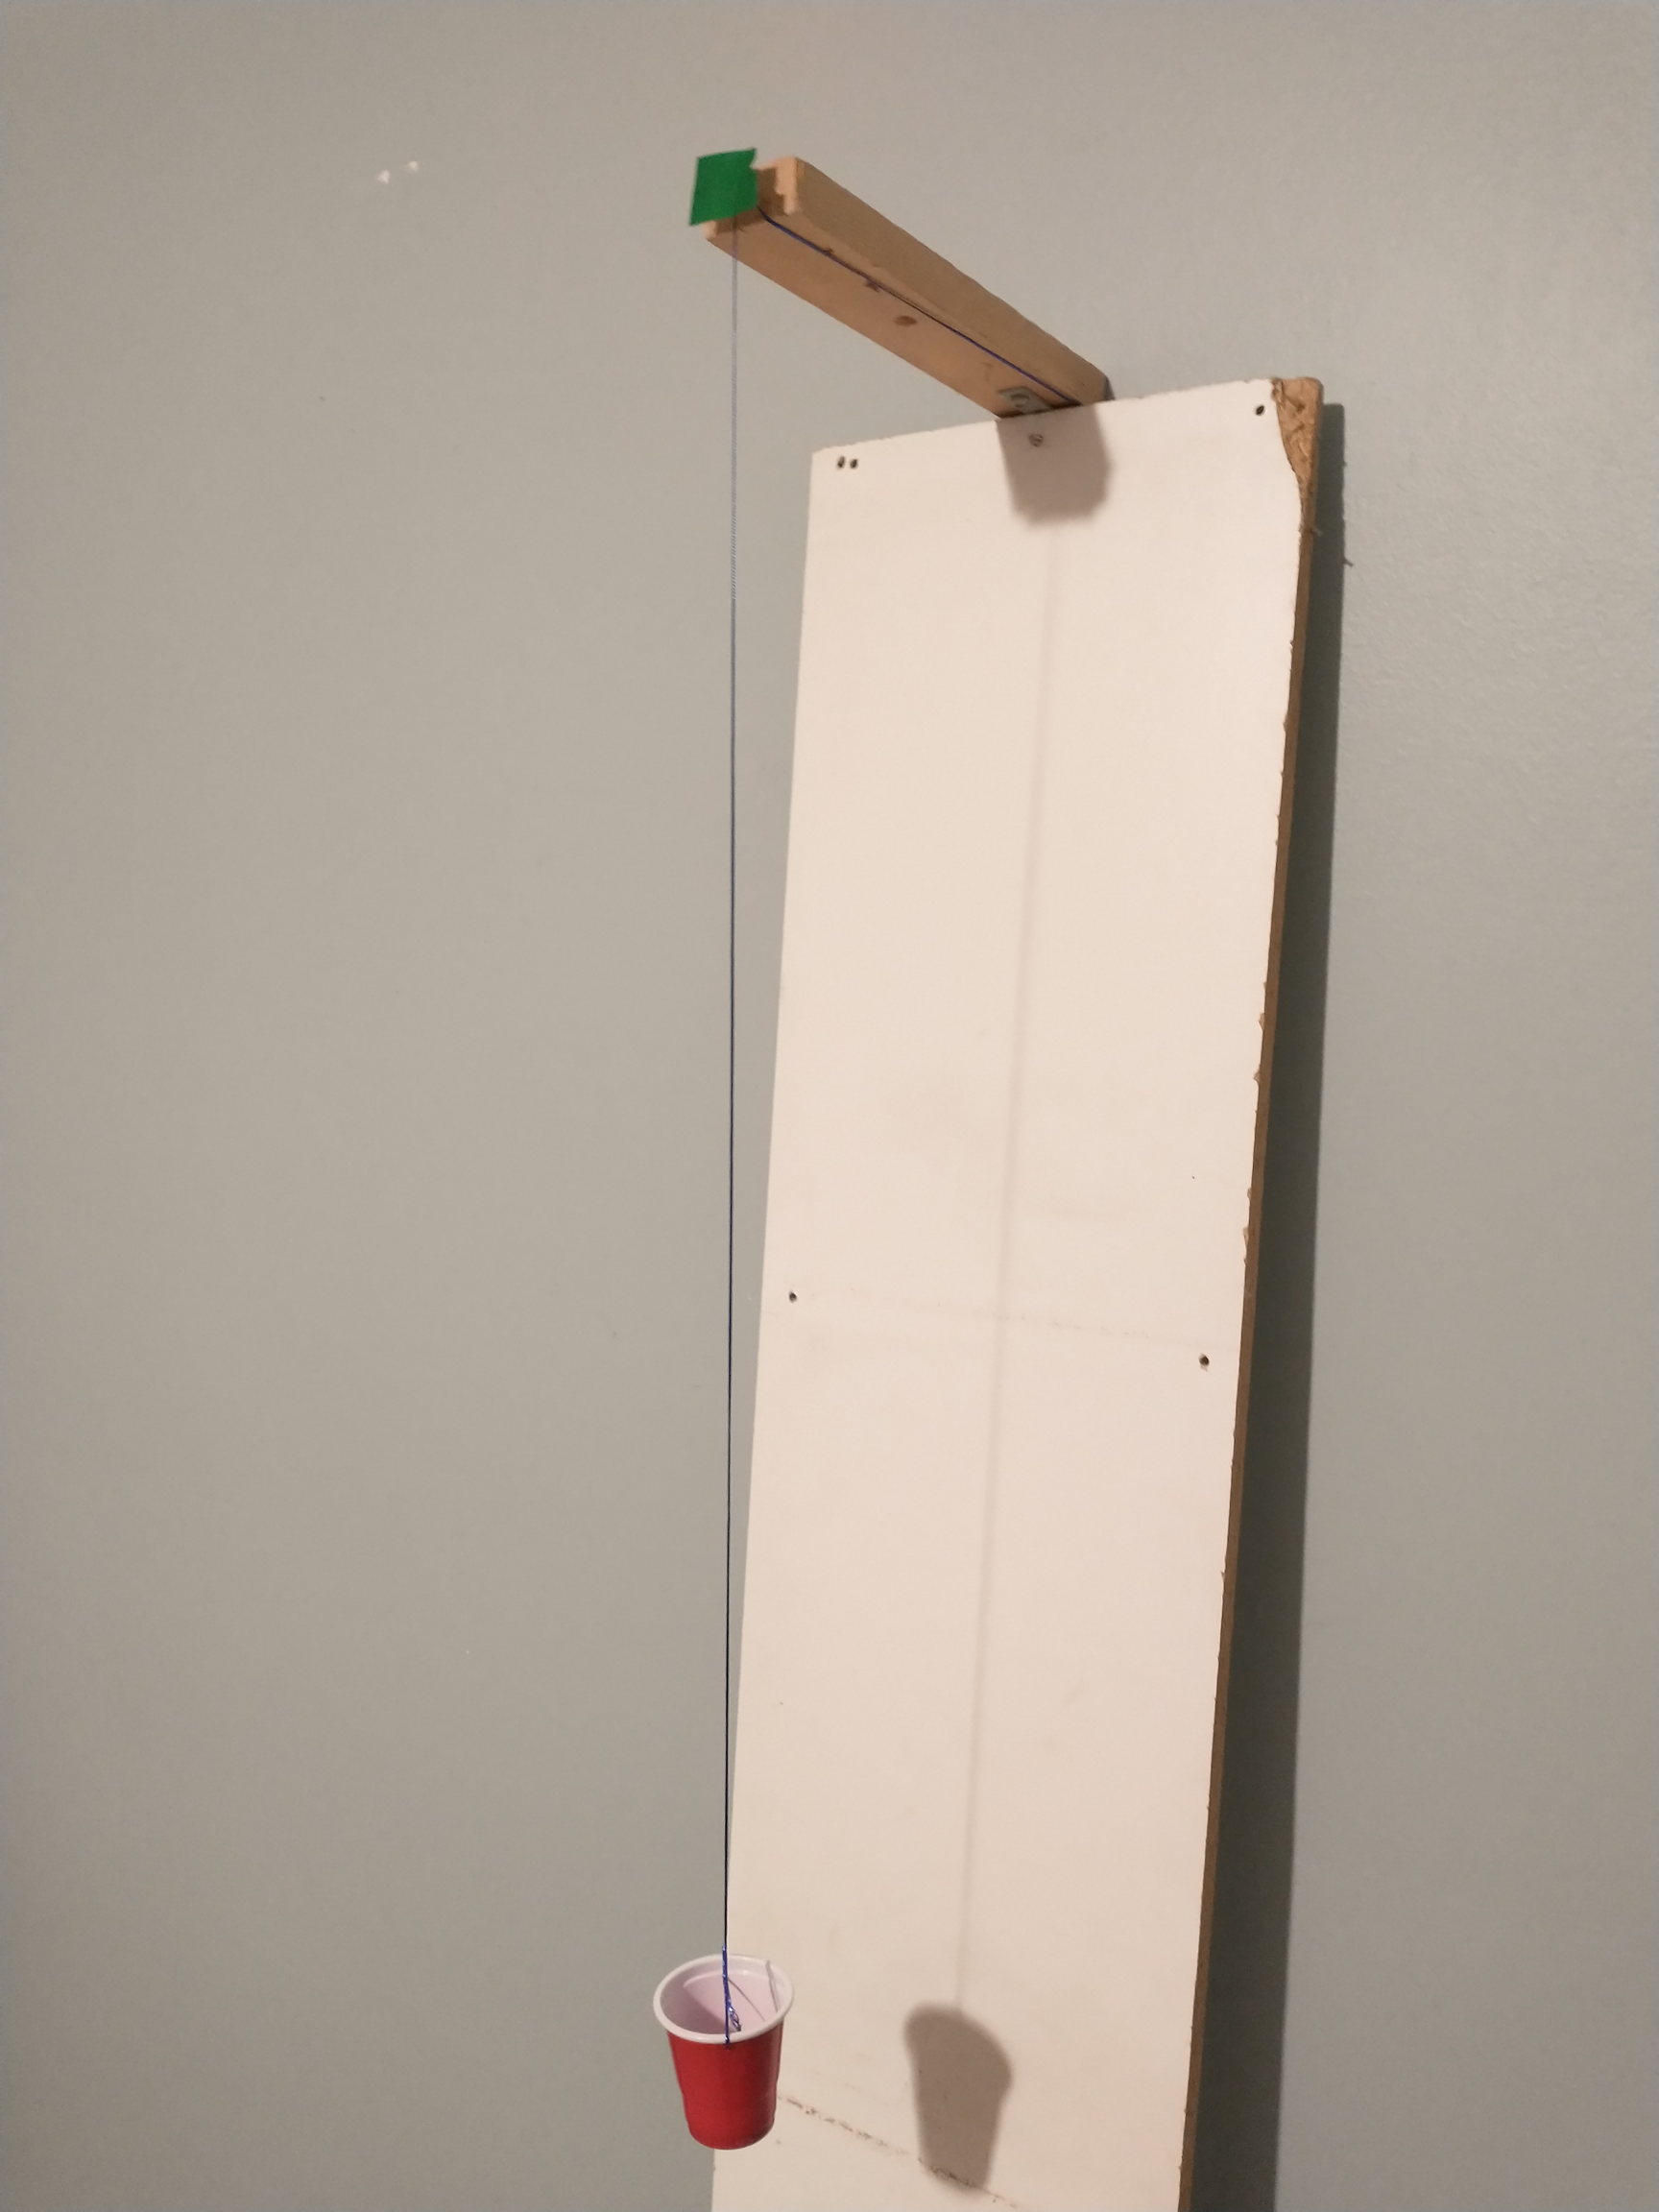
\includegraphics[width=0.6\linewidth]{pendulum.png}
    \caption{The pendulum constructed for this experiment.}
\end{figure}

The main support structure of the pendulum consists of two pieces of wood, attached together with screws and an
L-bracket. This was chosen because the material was readily available, and could be substituted for any material of
similar size and suitable strength.

The string of the pendulum is a thin, braided string, specifically chosen for visibility and to minimize twisting in
order to keep the motion of the pendulum in the same plane. The string is wound around a screw at the top, with a piece
of green reflective tape on it for tracking.

The string is attached to a bob consisting of a small, red plastic cup with coins inside for weight. The colour of the
cup is deliberately chosen to allow for computer-vision (CV) based tracking. Coins are used for added weight because
they have known masses and are readily available.

The string length and bob mass are adjustable, but for this experiment, the distance from the pivot to the centre of the
mass is fixed at \(65\si{cm} \pm 1\si{cm}\), and the mass is fixed at 6 Canadian \$2 coins (about \(41.52\si{g}\)
assuming cup mass is negligible).

\subsection{Data Collection}
\label{section:method:data_collection}

\begin{figure}[htb]
    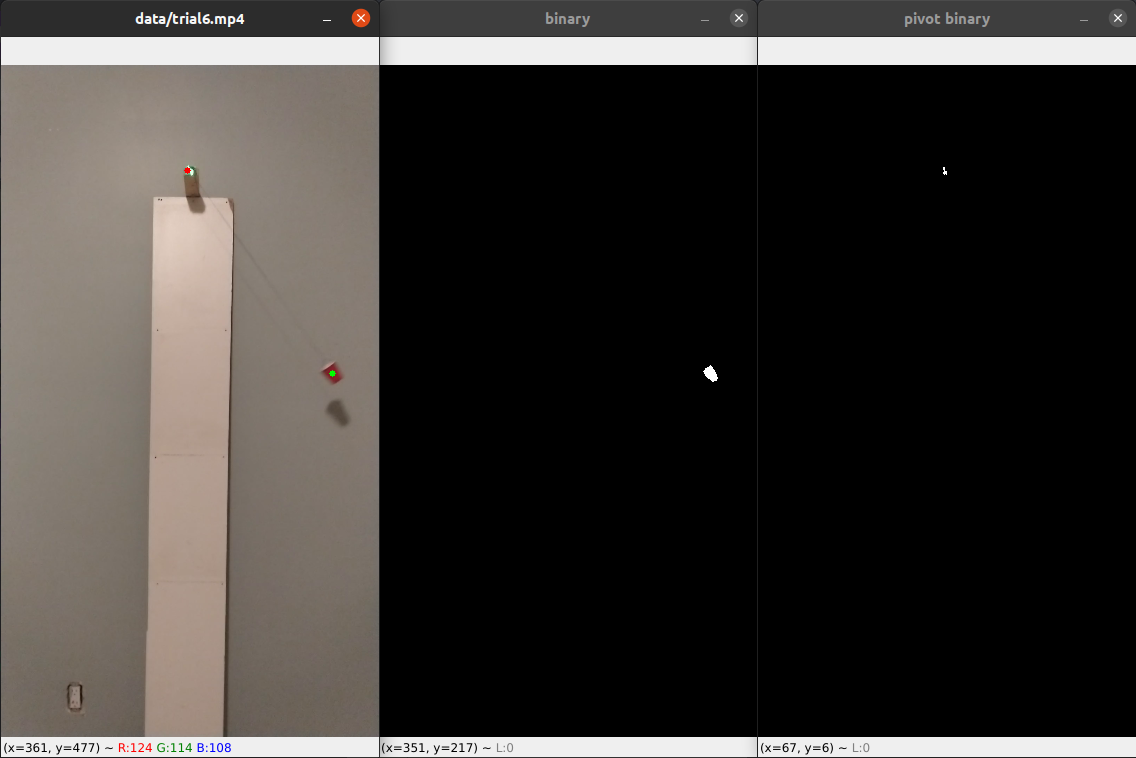
\includegraphics[width=\linewidth]{cv_track.png}
    \caption{CV-based tracking of the pendulum.}
\end{figure}

Videos of the pendulum are shot on a phone camera in FHD 60fps and then passed to a program to determine the angles.
The pendulum is released at a fixed starting amplitude each time, always starting on the right and swinging in the plane
of the camera.

The pendulum's angle is tracked using a Python program written with OpenCV (see Appendix \ref{appendix:code}).
The locations of the bob and pivot are determined by thresholding the image and then taking the average of the pixels to
find the centres. After the pixel coordinates have been determined, the ratio of the difference between the \(x\) and
\(y\) coordinates are used to compute the angle for each frame.

One data point is collected per 3 frames for 20 data points per second. Data collection starts as soon as the bob is
released, which is defined to be \(t = 0\).

\subsection{Data Analysis}

In total, 7 trials were conducted.
For each trial, the \(Q\) factor is determined using two independent methods as outlined below:

\subsubsection{Curve Fitting}

In the first method, \(Q\) is computed using Equation \ref{eqn:q} with values of \(\tau\) and \(T\) computed by fitting
Equation \ref{eqn:model} to the experimental data.

The data is passed to a Python program (see Appendix \ref{appendix:code}) that fits the model using a nonlinear
least-squares method, which determines the optimal values for \(\tau\) and \(T\) among others, and the standard
deviations of both, which is used as the uncertainty.

\subsubsection{Oscillation Counting}
\label{section:method:oscillation}

In the second method, the number of oscillations until the amplitude decays to \(e^{-\pi/3}\) of the original is
counted, which corresponds to \(\frac{Q}{3}\). The counting is again done with a Python program (see Appendix
\ref{appendix:code}).

Note that here an "oscillation" is defined as one complete period of the pendulum's swing. "Half-oscillations" are
counted if the amplitude first reaches the target value without completing a full period. For example, if the pendulum
starts at all the way to the right, and first reaches the target amplitude when it is swinging all the way to the left,
then a half-oscillation will be counted for the last cycle.

%%%%%%%%%%%%%%%%%%%%%%%%%%%%%%%%%%%%%%%%%%%%%%%%%%%%%%%%%%%%%%%%%%

\section{Observations}

\subsection{Curve Fitting}

\begin{figure*}[htb]
    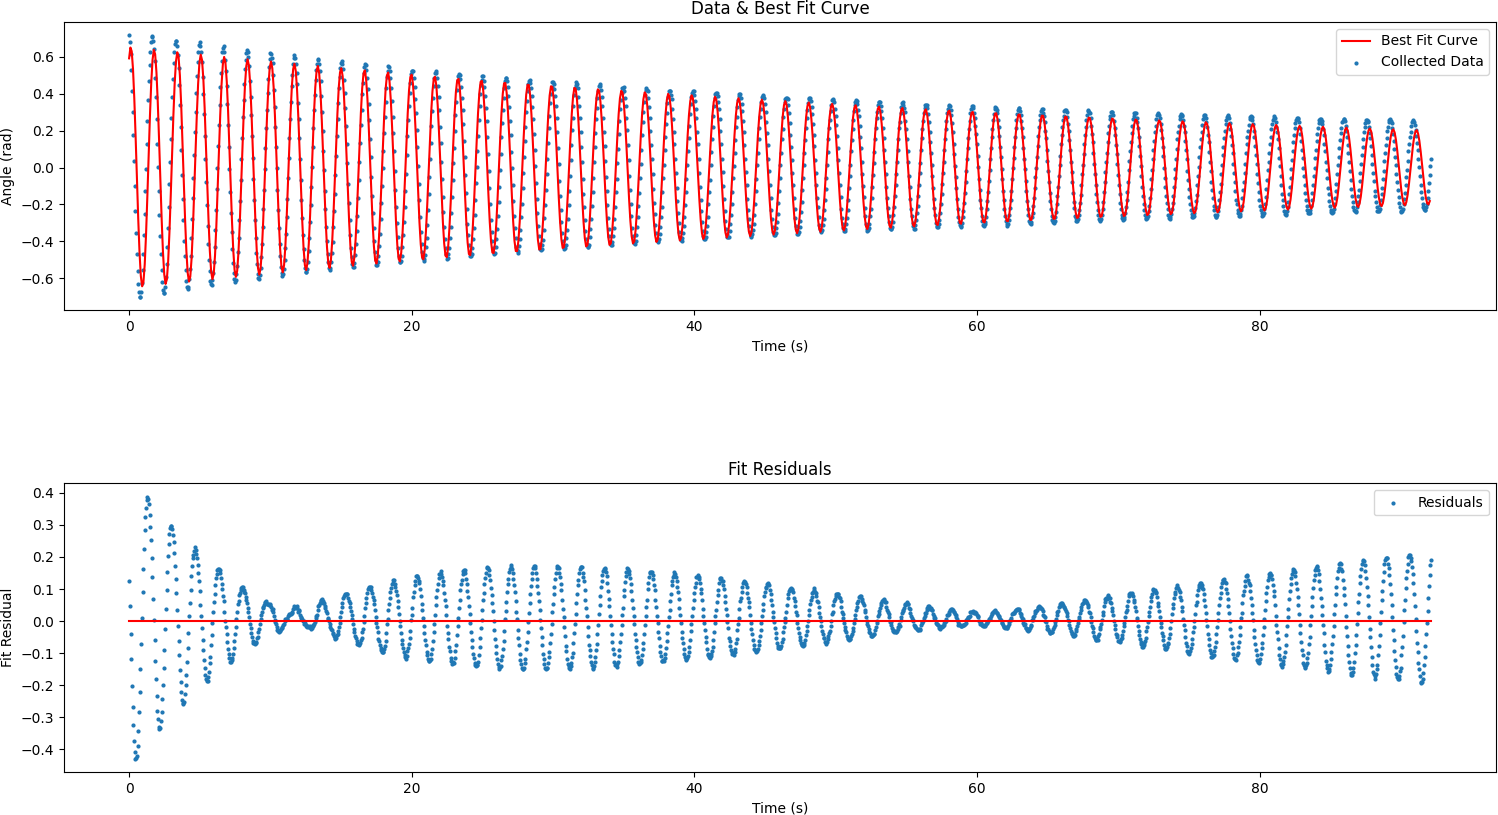
\includegraphics[width=0.725\linewidth]{fit1.png}
    \caption{Result of fitting Equation \ref{eqn:model} to the data. For this particular fit, \(A = 0.653\),
    \(\tau = 77.9\), \(T = 1.65\), \(\phi = -0.439\). Uncertainty bars are omitted to improve readability.}
    \label{fig:fit}
    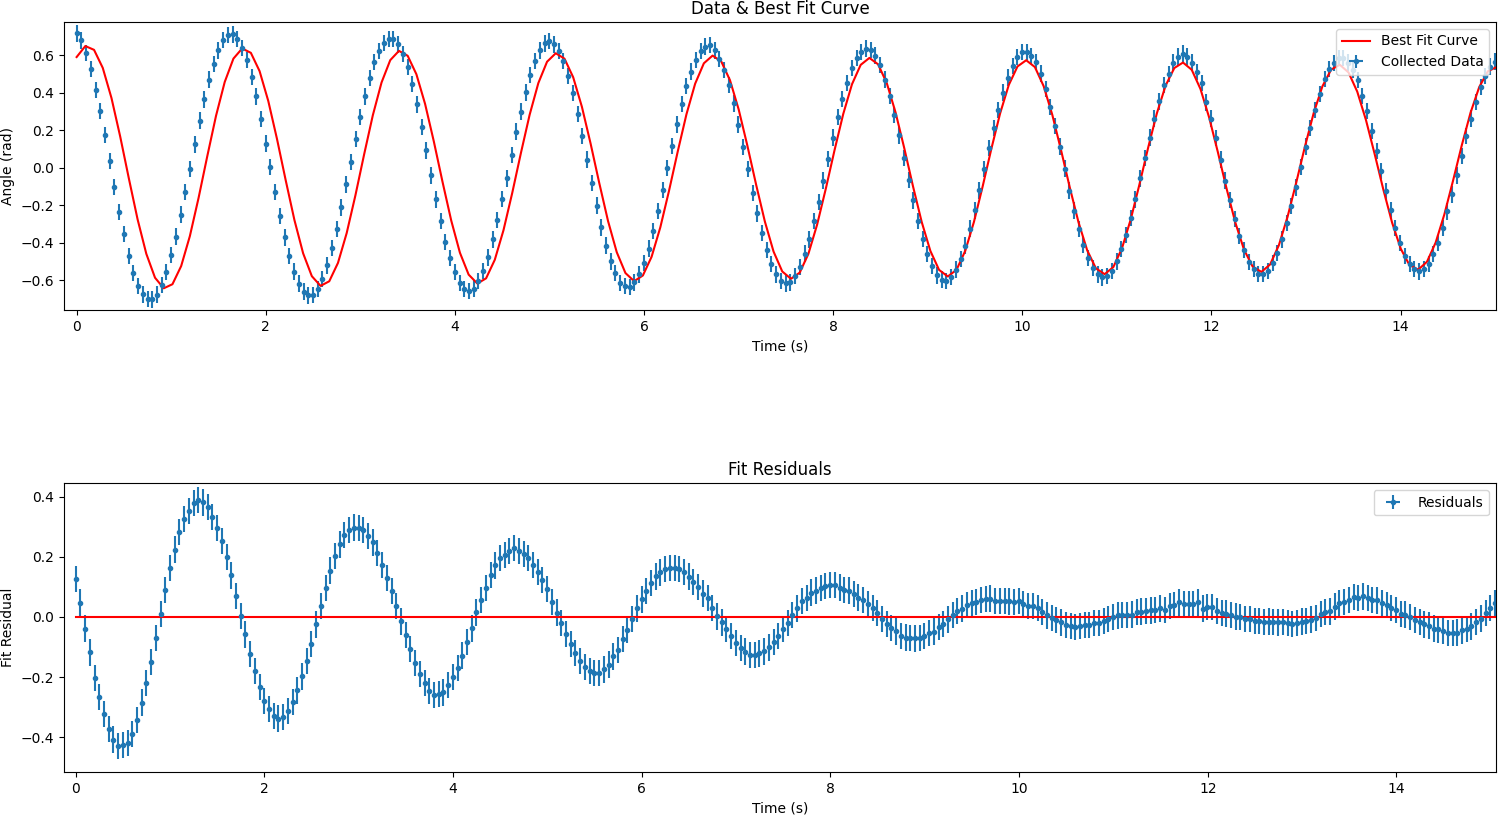
\includegraphics[width=0.725\linewidth]{fit2.png}
    \caption{Zoomed in view of the first 15 seconds.}
    \label{fig:fitzoom}
\end{figure*}

\(Q\) values computed using this method are shown in Table \ref{table:fit}:
\begin{table}[h]
    \begin{tabular}{c|c|c|c}
        Trial & \(Q\) & Uncertainty & \% Uncertainty \\
        \hline
        1   & 153.23    & \(\pm 3.65\) & 2.38 \\
        2   & 147.89    & \(\pm 3.95\) & 2.67 \\
        3	& 140.96	& \(\pm 3.53\) & 2.51 \\
        4	& 151.12	& \(\pm 3.81\) & 2.52 \\
        5	& 130.24	& \(\pm 3.86\) & 2.96 \\
        6	& 131.31	& \(\pm 3.76\) & 2.86 \\
        7	& 138.04	& \(\pm 3.70\) & 2.68 \\
        \hline
        \multicolumn{3}{l}{Mean} & 141.83 \\
        \multicolumn{3}{l}{Standard Deviation} & 9.24 \\
        \multicolumn{3}{l}{Uncertainty of the Mean} & 3.49
    \end{tabular}
    \caption{Raw data from curve fitting; values are \textbf{unrounded}. For final uncertainties see Section
        \ref{section:uncertainty}.}
    \label{table:fit}
\end{table}

A graph of the data and curve fit for one trial is shown in Figure \ref{fig:fit} and Figure \ref{fig:fitzoom}.

\subsection{Oscillation Counting}

\(Q\) values computed using this method are shown in Table \ref{table:oscillation}:
\begin{table}[h]
    \begin{tabular}{c|c|c|c}
        Trial & \(Q\) & Uncertainty & \% Uncertainty \\
        \hline
        1   & 148.5 & \(\pm 1.5\) & 1.01 \\
        2   & 151.5 & \(\pm 1.5\) & 0.99 \\
        3	& 148.5 & \(\pm 1.5\) & 1.01 \\
        4	& 154.5 & \(\pm 1.5\) & 0.97 \\
        5	& 139.5 & \(\pm 1.5\) & 1.08 \\
        6	& 142.5 & \(\pm 1.5\) & 1.05 \\
        7	& 148.5 & \(\pm 1.5\) & 1.01 \\
        \hline
        \multicolumn{3}{l}{Mean} & 147.6 \\
        \multicolumn{3}{l}{Standard Deviation} & 5.11 \\
        \multicolumn{3}{l}{Uncertainty of the Mean} & 1.93
    \end{tabular}
    \caption{Raw data from oscillation counting; values are \textbf{unrounded}. For final uncertainties see Section
        \ref{section:uncertainty}.}
    \label{table:oscillation}
\end{table}

It was chosen to measure for \(\frac{Q}{3} \rightarrow e^{-\pi/3} \approx 0.3509\) because of the very high \(Q\)
factor of the pendulum. The data collected only covers a time range enough for \(\frac{Q}{3}\).

However, an interesting phenomenon can be observed by varying the fraction of \(Q\) to measure for.
For example, by measuring for \(\frac{Q}{4}\) instead, the data in Table \ref{table:oscillation4} is obtained.
\begin{table}[h]
    \begin{tabular}{c|c|c|c}
        Trial & \(Q\) & Uncertainty & \% Uncertainty \\
        \hline
        1   & 126.0 & \(\pm 2\) & 1.59 \\
        2   & 138.0 & \(\pm 2\) & 1.45 \\
        3	& 134.0 & \(\pm 2\) & 1.49 \\
        4	& 144.0 & \(\pm 2\) & 1.39 \\
        5	& 128.0 & \(\pm 2\) & 1.56 \\
        6	& 126.0 & \(\pm 2\) & 1.59 \\
        7	& 134.0 & \(\pm 2\) & 1.49 \\
        \hline
        \multicolumn{3}{l}{Mean} & 132.9 \\
        \multicolumn{3}{l}{Standard Deviation} & 6.72 \\
        \multicolumn{3}{l}{Uncertainty of the Mean} & 2.54
    \end{tabular}
    \caption{Data obtained from measuring \(\frac{Q}{4}\)} instead.
    \label{table:oscillation4}
\end{table}

After more trials, it can be observed that the value of \(Q\) observed through counting oscillations is dependent on the
fraction of \(Q\) that was measured for. Moreover, as the denominator increases, the observed \(Q\) value seems to
decrease, while according to the mathematical model the value of \(Q\) should be independent of the fraction measured.
This is likely because the model is not an accurate approximation of the actual system. (More details in Section
\ref{section:analysis}.)

\subsection{Uncertainty Analysis}
\label{section:uncertainty}

\subsubsection{Measurement Uncertainty}

There are two sources of measurement uncertainty during the data collection process that can be easily quantified:
\begin{enumerate}
    \item \textbf{Time measurement uncertainty from the camera's frame rate and shutter speed.} Because the camera only
          captures a set number of frames per second, this creates a small uncertainty about the exact time that data
          points occurred. An upper bound for this uncertainty can be obtained by taking the time between two frames and
          dividing by 2. For a 60fps camera, this results in an uncertainty of \(\pm 0.008\si{s}\).
    \item \textbf{Angle measurement uncertainty from motion blur and imperfect tracking.} Motion blur caused by a
          fast-moving bob can make the angle hard to measure, and imperfect computer vision tracking of the bob and
          pivot may also result in an incorrect angle. To estimate an upper bound of this uncertainty, a frame is taken
          from when the pendulum has its maximum velocity to maximize motion blur. Two lines are drawn representing the
          worst possible cases for tracking, and the angle between them is taken. The result is a range of about
          \(5\degree\), or an uncertainty of \(\pm 3\degree\)/\(\pm 0.05\si{rad}\).
\end{enumerate}
\begin{figure}[h]
    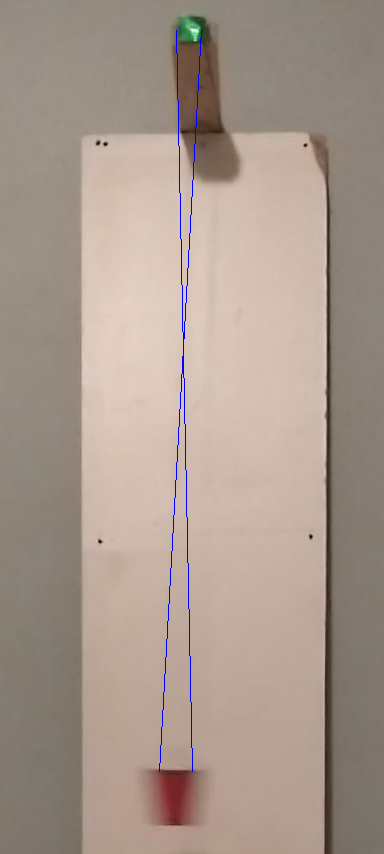
\includegraphics[width=0.3\linewidth]{uncert1.png}
    \caption{Worst-case scenarios for angle uncertainty. Blue lines are drawn to indicate the greatest and least
        possible angle.}
\end{figure}

These uncertainties are shown in the graphs in Figures \ref{fig:fit} and \ref{fig:fitzoom}. They are very small when
compared to the uncertainties later in the experiment, and so they will be ignored as only the largest uncertainty is
considered for this lab. Furthermore, their random nature means that these uncertainties would already be included in
the uncertainty of the mean.

There are also other sources of measurement uncertainty that are much harder to quantify:
\begin{enumerate}
    \item Perspective distortion
    \item Tilted camera
    \item Pendulum not swinging perfectly in the plane of the camera
\end{enumerate}
These uncertainties are assumed to be smaller and random, and thus incorporated in the uncertainty of the mean and other
sources described below.

\subsubsection{Uncertainties From Curve Fitting}

For each trial, the standard deviation obtained from the least squares fit is used as uncertainty values for \(\tau\)
and \(T\) and used to calculate uncertainty for \(Q\). From Table \ref{table:fit}, the greatest percentage uncertainty
is trial 5 with an uncertainty of 2.96\%. When multiplied by the mean, this corresponds to an uncertainty of
\(\pm 4.20\), which is greater than the uncertainty of the mean.

\textbf{The final value as determined by this method is \(Q = 142 \pm 4\).}

\subsubsection{Uncertainties From Oscillation Counting}

Since the amplitude can only be determined at the top of a peak or bottom of a trough, this method yields a maximum
resolution of 0.5 oscillations (half oscillations are allowed as described in Section \ref{section:method:oscillation}).

Because oscillations are counted until the amplitude first decays to less than the target instead of finding the cycle
with amplitude closest to the target, this yields an uncertainty of \(\pm 0.5\) oscillations, which corresponds to
\(\pm 1.5\) for the final \(Q\) value.

From Table \ref{table:oscillation}, the greatest percentage uncertainty is trial 5 with an uncertainty of 1.08\%, which
corresponds to an uncertainty of \(\pm 1.59\) in \(Q\), less than the uncertainty of the mean.

\textbf{The final value as determined by this method is \(Q = 148 \pm 2\).}

%%%%%%%%%%%%%%%%%%%%%%%%%%%%%%%%%%%%%%%%%%%%%%%%%%%%%%%%%%%%%%%%%%

\section{Analysis and Conclusion}
\label{section:analysis}

\subsection{\texorpdfstring{\(Q\)}{Q} Factor}

The \(Q\) value obtained by oscillation counting is within 1.5 times the uncertainty of the \(Q\) value obtained by
curve fitting. If values follow a normal distribution, there is a 13.4\% chance for values to be more than 1.5 times the
uncertainty away. From this we conclude that \textbf{while there is a discrepancy between the two \(Q\) values, there is
a chance that they are in agreement.} From the \(Q\) values and uncertainties alone, it can be concluded that the actual
\(Q\) value is between 142 and 148 and closer to the latter (since it has a lower uncertainty).

However, as shown in Table \ref{table:oscillation4}, by measuring for \(\frac{Q}{4}\) a \(Q\) value of \(133 \pm 3\) is
obtained instead. This value is 2.25 times the uncertainty away from the \(Q\) value obtained by curve fitting, and 5
times the uncertainty away from the \(Q\) value obtained by counting for \(\frac{Q}{3}\). The probability for a value to
lie outside 2.25 times the uncertainty is about 2.44\%, so this value is not in agreement with either \(Q\) value found
above.

Furthermore, as the fraction of \(Q\) measured for gets smaller, the measured \(Q\) value gets even further from the
values obtained previously. It can be concluded that, at least for this particular pendulum, \textbf{oscillation
counting is not a reliable way for obtaining \(Q\)}.

\subsection{Model Accuracy}

An inspection of the residuals in Figure \ref{fig:fit} shows a clear pattern, which would not be present if the fit
represented the data well. At many points, the residuals reach a value of 0.2, which is over 25\% of the actual
amplitude of the data, 0.8. The amplitude of the fit also deviates significantly from the actual amplitude of the data
(0.6 versus 0.8), but adjusting the conditions of the fit does not improve it.

The two possible reasons for this happening are either that the fit was not done well, or the model does not reflect the
real data well. The data is inconclusive for determining which is the dominant effect, but there is likely \textbf{a mix
of both}.

The amplitudes obtained from fit seems to be systematically smaller than the actual peak amplitudes in the
data, which suggests an incorrect fit. However, it is also likely that the model itself is inaccurate: Due to the
experimental setup (see Section \ref{section:method:data_collection}), the theoretical value of \(\phi_0\) should
always be 0. However, all the trials have produced a nonzero value for \(\phi_0\).

Figure \ref{fig:fit_nophi} is the result of modifying the code to fix \(\phi\) at 0 (see Appendix \ref{appendix:code}).
\begin{figure}[htb]
    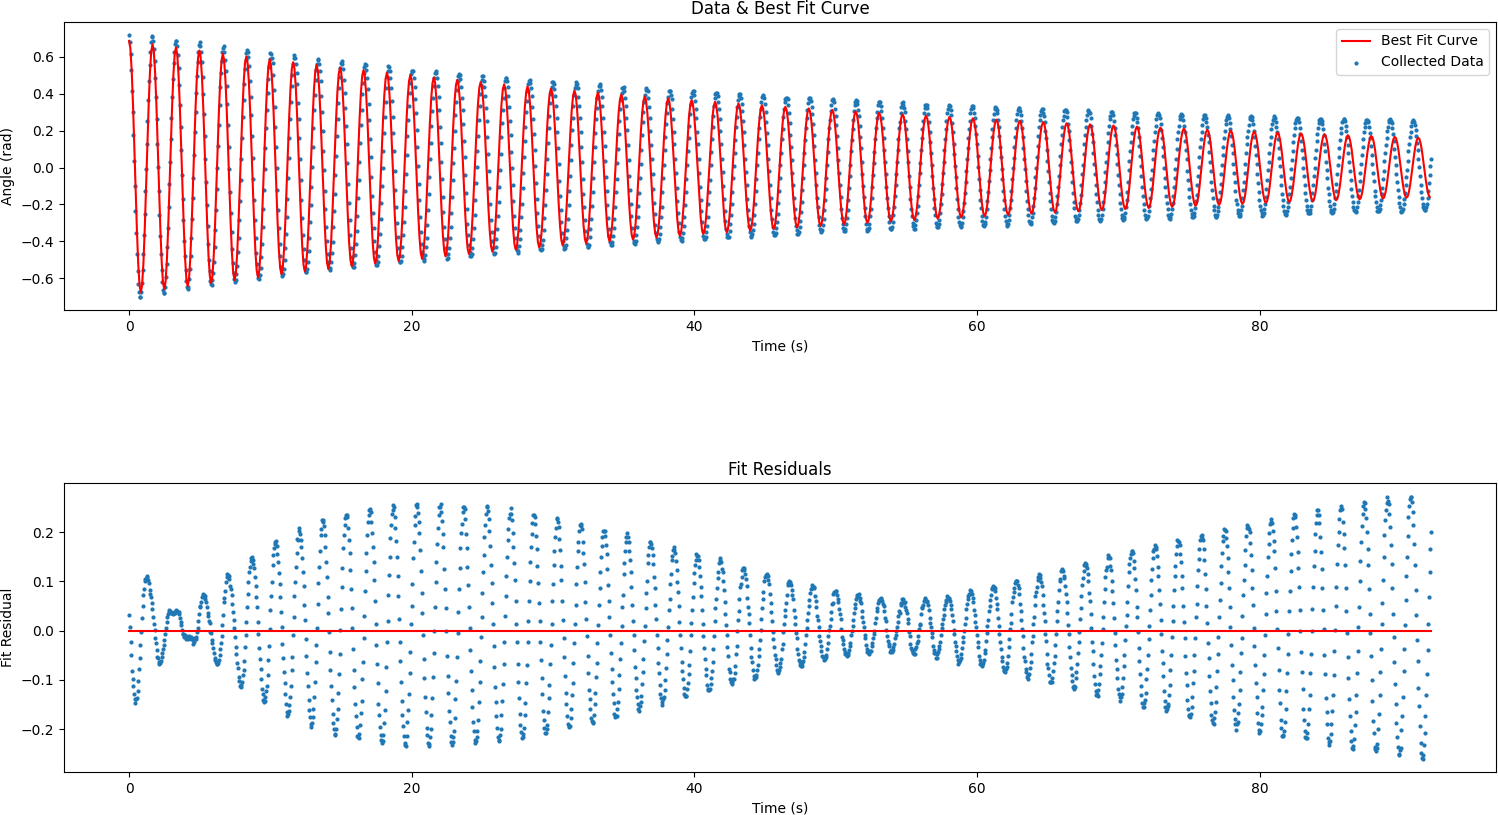
\includegraphics[width=0.9\linewidth]{fit3.png}
    \caption{Result of fitting Equation \ref{eqn:model} with \(\phi = 0\). For this particular fit, \(A = 0.686\),
    \(\tau = 63.16\), \(T = 1.66\). Uncertainty bars are omitted to improve readability.}
    \label{fig:fit_nophi}
\end{figure}

Compared to Figure \ref{fig:fit}, this time the fit is much worse, with the fit curve visibly deviating from the data in
both magnitude and phase near the end. The residuals seem to keep on increasing at the end, which allows us to conclude
that \textbf{Equation \ref{eqn:model} is likely not a very accurate model of this pendulum for large values of \(t\)}.

This might be because Equation \ref{eqn:model} is derived with the simplifying assumption of \(\sin x \approx x\) for
small angles and a damping force proportional to the velocity, while in reality drag is closer to quadratic.
This would cause the damping force to be stronger for smaller velocities, resulting in a rate of decay that is too fast
as shown in Figure \ref{fig:fit_nophi}.

For the fit in Figure \ref{fig:fit_nophi}, the largest percentage uncertainty was for the value of \(\tau\), which is
3.00\%. Assuming the 3.00\% carries over to the final value of \(\theta(t)\), this represents an uncertainty in the
worst case of \(\pm 0.0240\si{rad}\) (for a \(\theta\) value of 0.8). Comparing this to the residual graphs in Figures
\ref{fig:fit} and \ref{fig:fit_nophi}, the residuals easily exceed it by many times, even in regions where the
residuals are small.

Another reason for the large residuals could be that \textbf{the period of this pendulum appears to be non-constant}.
Observing the data more closely shows that the period of the pendulum appears to decrease slightly as time progresses.
In particular, for the trial in Figure \ref{fig:fit}, the initial period shortly after release is about
\(1.67\si{s} \pm 0.01\si{s}\), while the final period near the end of the video is about \(1.64\si{s} \pm 0.01\si{s}\).
Although the difference is small, it is consistently present throughout multiple trials and is too large to be explained
by uncertainties. This represents a slight deviation from the model, since Equation \ref{eqn:model} has a constant
period.

\subsection{Implications for Future Data Collection}

The findings have the following implications for data collection in future labs:
\begin{enumerate}
    \item The \(Q\) value was measured to be greater than 140, which means for every oscillation the amplitude decays to
          greater than \(e^{-\frac{\pi}{Q}} \approx 0.978 = 97.8\%\) of the previous oscillation. The high \(Q\) factor
          combined with a reasonably high period of about \(1.6\si{s}\) makes it very easy to measure multiple periods
          to get more accurate data, so in subsequent experiments more periods should be measured to improve accuracy.
    \item The slight change in period, although small (less than 2\%), means that results may differ depending on the
          when measurements are taken (specifically for measuring the period later in Lab 2). Therefore, special care
          should be taken to ensure that all period measurements are taken right at the beginning of the experiment so
          they could be compared.
\end{enumerate}

%%%%%%%%%%%%%%%%%%%%%%%%%%%%%%%%%%%%%%%%%%%%%%%%%%%%%%%%%%%%%%%%%%

\appendix
\section{Source Code}

A comprehensive list of all source code, as well as the \LaTeX{} source for this report, can be found on GitHub at
\url{https://github.com/tylertian123/phys180_lab}, in particular:
\label{appendix:code}
\begin{enumerate}
    \item For tracking the pendulum and generating time-angle data: \url{https://github.com/tylertian123/phys180_lab/blob/master/cvtrack.py}
    \item For fitting the model to experimental data: \url{https://github.com/tylertian123/phys180_lab/blob/master/fit.py}
    \item For measuring \(Q\) by counting oscillations: \url{https://github.com/tylertian123/phys180_lab/blob/master/find_q.py}
    \item For fitting the model with \(\phi\) fixed at 0: \url{https://github.com/tylertian123/phys180_lab/blob/master/fit_nophi.py}
\end{enumerate}

\end{document}
